\documentclass[twoside]{book}

% Packages required by doxygen
\usepackage{fixltx2e}
\usepackage{calc}
\usepackage{doxygen}
\usepackage[export]{adjustbox} % also loads graphicx
\usepackage{graphicx}
\usepackage[utf8]{inputenc}
\usepackage{makeidx}
\usepackage{multicol}
\usepackage{multirow}
\PassOptionsToPackage{warn}{textcomp}
\usepackage{textcomp}
\usepackage[nointegrals]{wasysym}
\usepackage[table]{xcolor}

% Font selection
\usepackage[T1]{fontenc}
\usepackage[scaled=.90]{helvet}
\usepackage{courier}
\usepackage{amssymb}
\usepackage{sectsty}
\renewcommand{\familydefault}{\sfdefault}
\allsectionsfont{%
  \fontseries{bc}\selectfont%
  \color{darkgray}%
}
\renewcommand{\DoxyLabelFont}{%
  \fontseries{bc}\selectfont%
  \color{darkgray}%
}
\newcommand{\+}{\discretionary{\mbox{\scriptsize$\hookleftarrow$}}{}{}}

% Page & text layout
\usepackage{geometry}
\geometry{%
  a4paper,%
  top=2.5cm,%
  bottom=2.5cm,%
  left=2.5cm,%
  right=2.5cm%
}
\tolerance=750
\hfuzz=15pt
\hbadness=750
\setlength{\emergencystretch}{15pt}
\setlength{\parindent}{0cm}
\setlength{\parskip}{3ex plus 2ex minus 2ex}
\makeatletter
\renewcommand{\paragraph}{%
  \@startsection{paragraph}{4}{0ex}{-1.0ex}{1.0ex}{%
    \normalfont\normalsize\bfseries\SS@parafont%
  }%
}
\renewcommand{\subparagraph}{%
  \@startsection{subparagraph}{5}{0ex}{-1.0ex}{1.0ex}{%
    \normalfont\normalsize\bfseries\SS@subparafont%
  }%
}
\makeatother

% Headers & footers
\usepackage{fancyhdr}
\pagestyle{fancyplain}
\fancyhead[LE]{\fancyplain{}{\bfseries\thepage}}
\fancyhead[CE]{\fancyplain{}{}}
\fancyhead[RE]{\fancyplain{}{\bfseries\leftmark}}
\fancyhead[LO]{\fancyplain{}{\bfseries\rightmark}}
\fancyhead[CO]{\fancyplain{}{}}
\fancyhead[RO]{\fancyplain{}{\bfseries\thepage}}
\fancyfoot[LE]{\fancyplain{}{}}
\fancyfoot[CE]{\fancyplain{}{}}
\fancyfoot[RE]{\fancyplain{}{\bfseries\scriptsize Generated by Doxygen }}
\fancyfoot[LO]{\fancyplain{}{\bfseries\scriptsize Generated by Doxygen }}
\fancyfoot[CO]{\fancyplain{}{}}
\fancyfoot[RO]{\fancyplain{}{}}
\renewcommand{\footrulewidth}{0.4pt}
\renewcommand{\chaptermark}[1]{%
  \markboth{#1}{}%
}
\renewcommand{\sectionmark}[1]{%
  \markright{\thesection\ #1}%
}

% Indices & bibliography
\usepackage{natbib}
\usepackage[titles]{tocloft}
\setcounter{tocdepth}{3}
\setcounter{secnumdepth}{5}
\makeindex

% Hyperlinks (required, but should be loaded last)
\usepackage{ifpdf}
\ifpdf
  \usepackage[pdftex,pagebackref=true]{hyperref}
\else
  \usepackage[ps2pdf,pagebackref=true]{hyperref}
\fi
\hypersetup{%
  colorlinks=true,%
  linkcolor=blue,%
  citecolor=blue,%
  unicode%
}

% Custom commands
\newcommand{\clearemptydoublepage}{%
  \newpage{\pagestyle{empty}\cleardoublepage}%
}

\usepackage{caption}
\captionsetup{labelsep=space,justification=centering,font={bf},singlelinecheck=off,skip=4pt,position=top}

%===== C O N T E N T S =====

\begin{document}

% Titlepage & ToC
\hypersetup{pageanchor=false,
             bookmarksnumbered=true,
             pdfencoding=unicode
            }
\pagenumbering{roman}
\begin{titlepage}
\vspace*{7cm}
\begin{center}%
{\Large P\+ID Controller }\\
\vspace*{1cm}
{\large Generated by Doxygen 1.8.11}\\
\end{center}
\end{titlepage}
\clearemptydoublepage
\tableofcontents
\clearemptydoublepage
\pagenumbering{arabic}
\hypersetup{pageanchor=true}

%--- Begin generated contents ---
\chapter{Class Index}
\section{Class List}
Here are the classes, structs, unions and interfaces with brief descriptions\+:\begin{DoxyCompactList}
\item\contentsline{section}{\hyperlink{classPID__Controller}{P\+I\+D\+\_\+\+Controller} }{\pageref{classPID__Controller}}{}
\end{DoxyCompactList}

\chapter{File Index}
\section{File List}
Here is a list of all documented files with brief descriptions\+:\begin{DoxyCompactList}
\item\contentsline{section}{app/\hyperlink{pid__controller_8cpp}{pid\+\_\+controller.\+cpp} \\*P\+ID controller class implementation }{\pageref{pid__controller_8cpp}}{}
\item\contentsline{section}{include/{\bfseries pid\+\_\+controller.\+hpp} }{\pageref{pid__controller_8hpp}}{}
\end{DoxyCompactList}

\chapter{Class Documentation}
\hypertarget{classPID__Controller}{}\section{P\+I\+D\+\_\+\+Controller Class Reference}
\label{classPID__Controller}\index{P\+I\+D\+\_\+\+Controller@{P\+I\+D\+\_\+\+Controller}}
\subsection*{Public Member Functions}
\begin{DoxyCompactItemize}
\item 
double \hyperlink{classPID__Controller_aca7348d8985a014f7684dabd422403e1}{compute\+\_\+velocity} (double set\+\_\+point, double target\+\_\+vel)
\begin{DoxyCompactList}\small\item\em Computes the velocity for the P\+ID controller. \end{DoxyCompactList}\end{DoxyCompactItemize}


\subsection{Member Function Documentation}
\index{P\+I\+D\+\_\+\+Controller@{P\+I\+D\+\_\+\+Controller}!compute\+\_\+velocity@{compute\+\_\+velocity}}
\index{compute\+\_\+velocity@{compute\+\_\+velocity}!P\+I\+D\+\_\+\+Controller@{P\+I\+D\+\_\+\+Controller}}
\subsubsection[{\texorpdfstring{compute\+\_\+velocity(double set\+\_\+point, double target\+\_\+vel)}{compute_velocity(double set_point, double target_vel)}}]{\setlength{\rightskip}{0pt plus 5cm}double P\+I\+D\+\_\+\+Controller\+::compute\+\_\+velocity (
\begin{DoxyParamCaption}
\item[{double}]{set\+\_\+pt, }
\item[{double}]{target\+\_\+velocity}
\end{DoxyParamCaption}
)}\hypertarget{classPID__Controller_aca7348d8985a014f7684dabd422403e1}{}\label{classPID__Controller_aca7348d8985a014f7684dabd422403e1}


Computes the velocity for the P\+ID controller. 


\begin{DoxyParams}{Parameters}
{\em set} & point and the target velocity \\
\hline
\end{DoxyParams}
\begin{DoxyReturn}{Returns}
computed velocity 
\end{DoxyReturn}


The documentation for this class was generated from the following files\+:\begin{DoxyCompactItemize}
\item 
include/pid\+\_\+controller.\+hpp\item 
app/\hyperlink{pid__controller_8cpp}{pid\+\_\+controller.\+cpp}\end{DoxyCompactItemize}

\chapter{File Documentation}
\hypertarget{pid__controller_8cpp}{}\section{app/pid\+\_\+controller.cpp File Reference}
\label{pid__controller_8cpp}\index{app/pid\+\_\+controller.\+cpp@{app/pid\+\_\+controller.\+cpp}}


P\+ID controller class implementation.  


{\ttfamily \#include $<$iostream$>$}\\*
{\ttfamily \#include \char`\"{}../include/pid\+\_\+controller.\+hpp\char`\"{}}\\*
Include dependency graph for pid\+\_\+controller.\+cpp\+:
\nopagebreak
\begin{figure}[H]
\begin{center}
\leavevmode
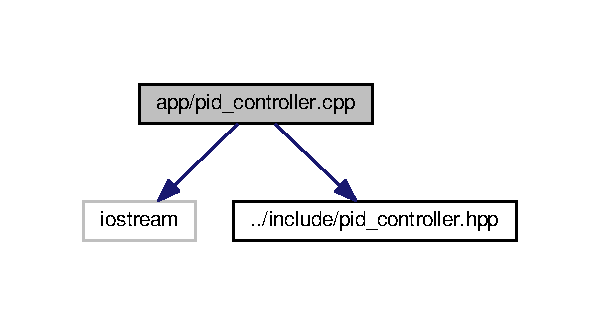
\includegraphics[width=288pt]{pid__controller_8cpp__incl}
\end{center}
\end{figure}


\subsection{Detailed Description}
P\+ID controller class implementation. 

Gautam Balachandran 
%--- End generated contents ---

% Index
\backmatter
\newpage
\phantomsection
\clearemptydoublepage
\addcontentsline{toc}{chapter}{Index}
\printindex

\end{document}
